\documentclass[12pt]{article}
\usepackage{amsmath}
\usepackage{graphicx}
\usepackage{siunitx}
\usepackage{float}
\usepackage{geometry}
\geometry{margin=1in}
\usepackage[utf8]{inputenc}
\usepackage{multicol}
\usepackage{xcolor}
\usepackage{subfigure}
\usepackage{titlesec}
\usepackage[bookmarks,breaklinks,colorlinks=true,allcolors=blue]{hyperref}
\usepackage{listings}
\usepackage{inconsolata}
\usepackage{eso-pic}
\usepackage[framemethod=tikz]{mdframed}
\usepackage[square,numbers]{natbib}
\usepackage{parskip}
\usepackage[official]{eurosym}
\usepackage{todonotes}
\usepackage{csquotes}
\usepackage{rotating}
\usepackage{lmodern}
\usepackage{setspace}
\usepackage{pdfpages}
\usepackage{svg}
\usepackage{hyperref} 
\lstset{
  language=Python,
  basicstyle=\ttfamily\small,
  keywordstyle=\color{blue},
  commentstyle=\color{gray},
  stringstyle=\color{orange},
  showstringspaces=false,
  breaklines=true,
  frame=single,
  captionpos=b,
  tabsize=4
}

\begin{document}
\begin{titlepage}
\begin{center}

\vspace*{1cm}

% Logo

\includegraphics[width=0.35\textwidth]{images/cedtnew.png}

\vspace{0.5cm}

{\Large \textbf{Centre for Electronic Design and Technology}}\\[0.25cm]
{\large Netaji Subhas University of Technology, New Delhi}

\vfill

% Title
{\Huge \textbf{Characterization of IR Photodiode}}\\[0.4cm]
{\Huge \textbf{Response to IR LED Illumination}}


\vspace{1.5cm}

% Authors
{\large \textbf{Submitted by}}\\[0.2cm]
{\large Ansh Gupta and Aditya Garg}\\

\vspace{0.8cm}

% Date
{\large \textbf{Date:} October 2024}

\vspace*{1cm}

\end{center}
\end{titlepage}

\clearpage
\pagenumbering{roman} 

\tableofcontents
\newpage

% ------------------------------
\section{Synopsis}

This experiment investigates the current response of IR photodiode to illumination from a IR LED under controlled optical isolation. The LED current was systematically varied, and the resulting photodiode current was measured using a digital multimeter. The experimental data, analyzed in Python, was fitted with a logistic model to capture the nonlinear response and saturation behavior. The results demonstrate the characteristic transition of the photodiode from its initial linear region to a saturation plateau, providing quantitative insight into IR photodiode operation.


% ------------------------------
\section{Introduction}

Infrared (IR) photodiodes are widely used in optoelectronic systems for detecting invisible infrared radiation. Their operation is based on the generation of photocurrent when incident IR photons are absorbed, making them suitable for applications such as remote controls, optical communication, proximity sensing, and reflective object detection. Unlike simple photoconductive elements, photodiodes exhibit a nonlinear current–light intensity relationship that depends on device geometry, wavelength sensitivity, and operating conditions. Accurately modeling this nonlinear behavior is crucial for designing reliable IR sensing circuits.

The aim of this experiment is to characterize the response of a IR photodiode as a function of the drive current through a IR LED. Since LED current can be treated as a proxy for optical irradiance, measuring the corresponding photodiode current allows us to establish a direct input–output relationship. By applying curve-fitting techniques, the experimental data is modeled with a logistic function, which captures both the initial rise and the saturation region of the photodiode response.

This study highlights the importance of empirical characterization in optical sensor systems. Even with relatively simple components such as IR LEDs and photodiodes, real-world data deviates from idealized linear assumptions, requiring accurate modeling to support sensor calibration, signal processing, and system-level design in IR-based applications.

\newpage
% ------------------------------
\section{Block Diagram}

\begin{figure}[H]
  \centering
  \fbox{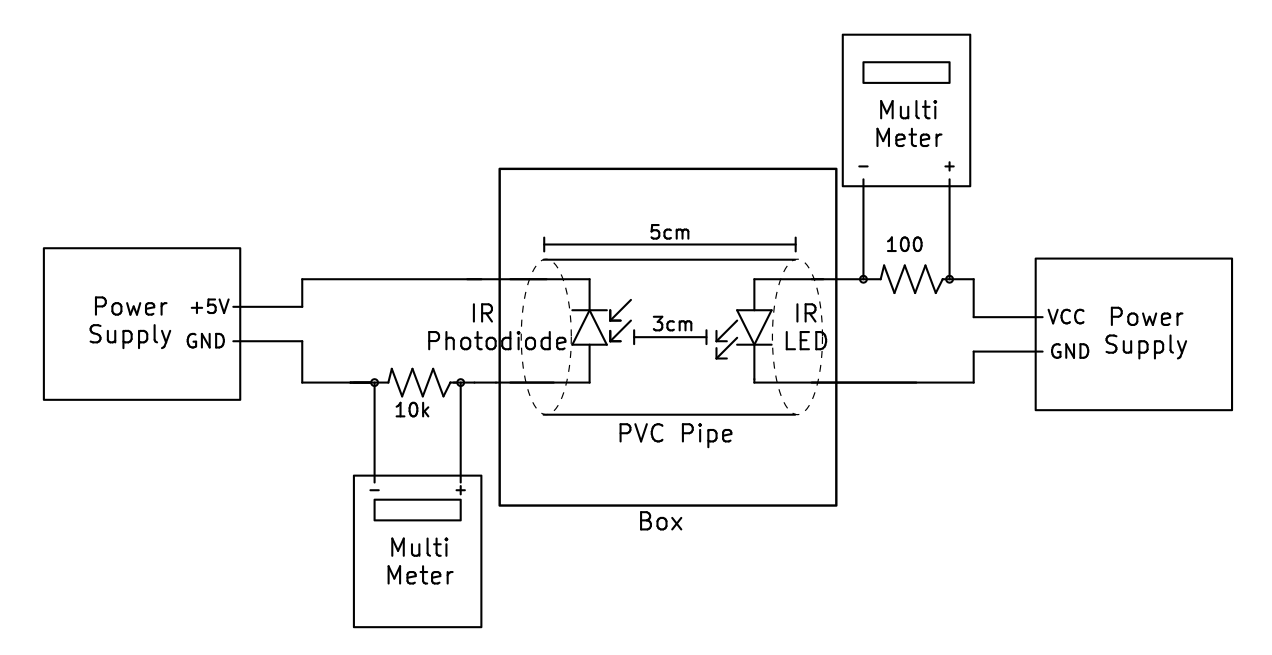
\includegraphics[width=1\textwidth]{images/Block_Diagram.png}}
  \caption{Block diagram of measurement setup.}
\end{figure}
\newpage
% ------------------------------
\section{Procedure}


 \begin{enumerate}
  \item \textbf{Optical Isolation Setup:} A \SI{5}{\milli\meter} IR LED and  IR photodiode were mounted facing each other inside a black PVC tube of \SI{1}{\inch} diameter and \SI{5}{\centi\meter} length. To ensure complete optical isolation, the tube was wrapped with multiple layers of black tape, making it fully opaque to ambient light.

  \item \textbf{Mechanical Alignment:} Both the IR LED and photodiode were centered and fixed in position, maintaining a constant separation of \SI{3}{\centi\meter} throughout the experiment.

  \item \textbf{LED Current Control:} A dual DC power supply was used to bias the LED and photodiode independently. The IR LED was driven by a variable DC output, and its current was monitored by measuring the voltage drop across a precision \SI{100}{\ohm} series resistor using a digital multimeter.

  \item \textbf{Photodiode Reverse Bias and Current Measurement:} The photodiode was connected in reverse bias using a regulated \SI{5}{\volt} DC supply. Its output current was measured by recording the voltage drop across a \SI{10}{\kilo\ohm} load resistor with a second multimeter, ensuring accurate current readings.

  \item \textbf{Stabilized Measurements:} For each LED current value, the corresponding photodiode current was allowed to stabilize before recording to minimize transient errors.

  \item \textbf{Dark Enclosure:} The entire LED–photodiode assembly was placed inside a closed cardboard box to eliminate stray light interference and ensure consistent optical conditions.

  \item \textbf{Data Logging:} Photodiode current values corresponding to different LED drive currents were tabulated and stored in a CSV file for further analysis.

  \item \textbf{Curve Fitting:} The recorded data was analyzed in Python using a logistic model of the form
  \[
  I_{\text{PD}} = \frac{I_{\text{sat}}}{1 + e^{-\alpha (I_{\text{LED}} - I_0)}}
  \]
  where \( I_{\text{PD}} \) is the photodiode current, \( I_{\text{LED}} \) is the LED drive current, and \( I_{\text{sat}}, \alpha, I_0 \) are fitting parameters.
\end{enumerate}


\newpage
% ------------------------------
\section{Model Fitting and Analysis}

The photodiode response shows a rapid increase at low LED currents and saturates at high currents. To quantify this behavior, a logistic model was employed:

\[
I_{PD} = \frac{I_{sat}}{1 + e^{-\alpha (I_{LED} - I_0)}}
\]

where:
\begin{itemize}
  \item $I_{PD}$: Photodiode current (\si{\micro\ampere})
  \item $I_{LED}$: LED current (\si{\micro\ampere})
  \item $I_{sat}$: Saturation current (\si{\micro\ampere})
  \item $\alpha$: Steepness of the response (per µA)
  \item $I_0$: Midpoint LED current corresponding to half-saturation (\si{\micro\ampere})
\end{itemize}

The logistic curve was fitted to the experimental data using \texttt{scipy.optimize.curve\_fit} to determine $I_{sat}$, $\alpha$, and $I_0$. The fit accurately captures the saturation behavior and the nonlinear growth at low LED currents.



% ------------------------------
\section{Results}

The measured photodiode current was plotted against LED current. The response shows a rapid increase at low LED currents and saturates at approximately 510\,µA at high LED currents.  

\begin{figure}[H]
  \centering
  \includesvg[width=1.0\textwidth]{images/ir_plot}
  \caption{IR Photodiode Response vs IR LED Current.}
  \label{fig:IR_PD}
\end{figure}

The logistic model fit the experimental data with parameters:

\[
I_{PD} = \frac{510.79}{1 + e^{-0.00055 (I_{LED} - 416.07)}}
\]

where $I_{PD}$ and $I_{LED}$ are in µA.

\newpage
% ------------------------------
\section{Conclusion}

The experiment successfully demonstrated the nonlinear response of a \SI{5}{\milli\meter} IR photodiode to illumination from a \SI{5}{\milli\meter} IR LED. By isolating the LED–photodiode pair inside a black PVC tube and enclosing the setup within a cardboard box, stable current measurements were obtained across a wide range of LED drive currents.  

The measured data showed clear saturation behavior, and the logistic model provided an excellent fit to the photodiode response. The fitted parameters were:  
\[
I_{\text{sat}} = 508.0 \, \mu\text{A}, \quad 
\alpha = 0.01588 \, \mu\text{A}^{-1}, \quad
I_{0} = 219.96 \, \mu\text{A}.
\]

This model accurately captures both the rapid growth in photodiode current at low LED currents and the saturation plateau at higher currents. The extracted parameters offer a quantitative basis for sensor calibration and can be directly applied to the design of optical sensing systems where photodiode linearity and saturation must be considered.


% ------------------------------


\section{Bill of Material}

\begin{table}[H]
\centering
\begin{tabular}{|c|l|l|c|}
\hline
\textbf{S No.} & \textbf{Component} & \textbf{Value} & \textbf{Quantity} \\ \hline
1  & IR Photodiode & 5mm & 1 \\
2 &  IR LED & 5mm($\lambda_p = 940$\,nm, $V_f = 1.228$\,V)  & 1\\
3 & Resistor & \SI{10}{\kilo\ohm} & 1\\
3 & Resistor & \SI{100}{\ohm} & 1\\
4 & Digital Multimeter & -  & 1 \\
5 & PVC pipe & 2.5cm x 5cm  & 1  \\
6 & Cardboard Box & 15cm x 14cm &  1  \\

\hline
\end{tabular}
\caption{Components used in the  experiment}
\end{table}


\section{Appendix}
\subsection*{Data File}
\begin{itemize}
  \item \href{https://drive.google.com/drive/folders/1A5ta1QYY_Sygo3tfl44TySLrXgKUCzGN?usp=drive_link} {IR Photodiode Characteristics.csv}
\end{itemize}
\subsection*{Code Files}
\begin{itemize}
  \item \href{https://drive.google.com/drive/folders/1DQeljcbbAsHtRlvSBTwIV61tD_d72g0o?usp=drive_link}{Python Code}
\end{itemize}

\end{document}



